\documentclass[UTF8,a4paper,10pt,nocolorlinks]{ctexart}
\usepackage[left=2.50cm, right=2.50cm, top=2.50cm, bottom=2.50cm]{geometry} %页边距
\CTEXsetup[format={\Large\bfseries}]{section} %设置章标题居左   


\usepackage{setspace}
\usepackage{xcolor}
\usepackage{mdframed}
\usepackage{titletoc}
\usepackage{etoolbox}
%%%%%%%%%%%%%%%%%%%%%%%
% -- text font --
% compile using Xelatex
%%%%%%%%%%%%%%%%%%%%%%%
% -- 中文字体 --
%\setmainfont{Microsoft YaHei}  % 微软雅黑
%\setmainfont{YouYuan}  % 幼圆    
%\setmainfont{NSimSun}  % 新宋体
%\setmainfont{KaiTi}    % 楷体
%\setmainfont{SimSun}   % 宋体
%\setmainfont{SimHei}   % 黑体
% -- 英文字体 --
%\usepackage{times}
%\usepackage{mathpazo}
%\usepackage{fourier}
%\usepackage{charter}
\usepackage{helvet}
\usepackage{caption}
\usepackage{multicol} %用于实现在同一页中实现不同的分栏
\usepackage{changepage}
\usepackage{graphics}
\usepackage{amsmath, amsfonts, amssymb} % math equations, symbols
\usepackage[english]{babel}
\usepackage{color}      % color content
\usepackage{graphicx}   % import figures
\usepackage{url}        % hyperlinks
\usepackage{bm}         % bold type for equations
\usepackage{multirow}
\usepackage{booktabs}
\usepackage{epstopdf}
\usepackage{epsfig}
\usepackage{algorithm}
\usepackage{algorithmic}
\newcommand{\sihao}{\fontsize{14pt}{\baselineskip}}
\renewcommand{\algorithmicrequire}{ \textbf{Input:}}     % use Input in the format of Algorithm  
\renewcommand{\algorithmicensure}{ \textbf{Initialize:}} % use Initialize in the format of Algorithm  
\renewcommand{\algorithmicreturn}{ \textbf{Output:}}     % use Output in the format of Algorithm  
\renewcommand{\figurename}{图}
% 引用参考文献标号显示在右上角
\newcommand{\upcite}[1]{\textsuperscript{\textsuperscript{\cite{#1}}}}
% \hypersetup{colorlinks=false} 
% \usepackage{fancyhdr} %设置页眉、页脚
% %\pagestyle{fancy}
% \lhead{}
% \chead{}
% %\rhead{\includegraphics[width=1.2cm]{fig/ZJU_BLUE.eps}}
% \lfoot{}
% \cfoot{}
% \rfoot{} 
\usepackage{color}
\usepackage{subfigure}
\usepackage{changepage}
\usepackage{fancyhdr} %设置页眉、页脚
\pagestyle{fancy}  %%%单线页眉
\fancyhead{}
\fancyhead[LO]{chapter 9}
\fancyhead[RO]{fengxuewei}
% \fancyfoot[RO]{\thepage}
\fancypagestyle{plain}{%
  \pagestyle{fancy}
}
\usepackage{shorttoc}
\usepackage{xcolor}
\usepackage{mdframed}
\usepackage{titletoc}
\renewcommand{\today}{\CJKnumber\year 年 \CJKnumber\month 月 \CJKnumber\day 日}

\DeclareRobustCommand{\chuhao}{\fontsize{42pt}{\baselineskip}\selectfont}  % 初号
\DeclareRobustCommand{\xiaochu}{\fontsize{36pt}{\baselineskip}\selectfont} % 小初
\DeclareRobustCommand{\yihao}{\fontsize{26pt}{\baselineskip}\selectfont}   % 一号
\DeclareRobustCommand{\xiaoyi}{\fontsize{24pt}{\baselineskip}\selectfont}  % 小一
\DeclareRobustCommand{\erhao}{\fontsize{22pt}{\baselineskip}\selectfont}   % 二号
\DeclareRobustCommand{\xiaoer}{\fontsize{18pt}{\baselineskip}\selectfont}  % 小二
\DeclareRobustCommand{\sanhao}{\fontsize{16pt}{\baselineskip}\selectfont}  % 三号 
\DeclareRobustCommand{\xiaosan}{\fontsize{15pt}{\baselineskip}\selectfont} % 小三
\DeclareRobustCommand{\sihao}{\fontsize{14pt}{\baselineskip}\selectfont}   % 四号
\DeclareRobustCommand{\xiaosi}{\fontsize{12pt}{\baselineskip}\selectfont}  % 小四
\DeclareRobustCommand{\wuhao}{\fontsize{10.5pt}{\baselineskip}\selectfont} % 五号
\DeclareRobustCommand{\xiaowu}{\fontsize{9pt}{\baselineskip}\selectfont}   % 小五
\DeclareRobustCommand{\liuhao}{\fontsize{7.5pt}{\baselineskip}\selectfont} % 六号
\DeclareRobustCommand{\xiaoliu}{\fontsize{6.5pt}{\baselineskip}\selectfont}% 小六
\DeclareRobustCommand{\qihao}{\fontsize{5.5pt}{\baselineskip}\selectfont}  % 七号

\providecommand{\keywords}[1]{\textbf{\textit{keywords---}} #1}
%%%%%%%%%%%%%%%%%%%%%%%
%  设置水印
%%%%%%%%%%%%%%%%%%%%%%%
%\usepackage{draftwatermark}         % 所有页加水印
%\usepackage[firstpage]{draftwatermark} % 只有第一页加水印
% \SetWatermarkText{Water-Mark}           % 设置水印内容
% \SetWatermarkText{\includegraphics{fig/ZJDX-WaterMark.eps}}         % 设置水印logo
% \SetWatermarkLightness{0.9}             % 设置水印透明度 0-1
% \SetWatermarkScale{1}                   % 设置水印大小 0-1    
 
\usepackage{hyperref} %bookmarks

\captionsetup[figure]{labelfont={bf},labelformat={default},labelsep=period,name={图}}
\hypersetup{colorlinks, bookmarks, unicode} %unicode

\title{
    \textbf{chapter 9 Design Models for Guidance }\\
    \textbf{制导设计模型}
}
\author{ fengxuewei }
\date{\today}
\begin{document}
    \maketitle
    
    \begin{itemize}
        \item[(1)] 介绍连续闭环(SLC)方法
        \item[(2)] 执行器饱和度 saturation 及其对性能的限制
        \item[(3)] 横向自动飞行器的设计
        \item[(4)] 纵向自动飞行器的设计
        \item[(5)] 比例积分微分PID反馈控制
    \end{itemize}
    \clearpage
    \section{离心力}
    当物体在做非直线运动时(非牛顿环境,例如:圆周运动或转弯运动),
    因物体一定有本身的质量存在,
    质量造成的惯性会强迫物体继续朝着运动轨迹的切线方向(原来那一瞬间前进的直线方向)前进,
    而非顺着接下来转弯过去的方向走。
    \par 若这个在做非直线运动的物体(例如:车)上有乘客的话,乘客由于同样随着车子做转弯运动,
    会受到车子向乘客提供的向心力,但是若以乘客为参照系,由于该参照系为非惯性系,
    他会受到与他相对静止的车子给他的一个指向圆心的向心力作用,
    但同时他也会给车子一个反向等大,由圆心指向外的力,就好像没有车子他就要被甩出去一样,这个力就是所谓的离心力。
    \section{概念}
    \begin{itemize}
        \item[(1)] 
        航向角chi是地速相对于$i^{i}$(正北)方向的偏移角度, 偏航角yaw是空速方向; 在没有风的情况下, 偏航角和航向角是相等的
        \item[(2)] 升力是垂直副翼向上的
        \item[] 
        \item[(3)] roll的大小和方向: 机体坐标系OZb轴与通过机体OXb轴的铅垂面间的夹角,机体向右滚为正,反之为负。
        \item[(4)] $\gamma$是 地速方向和水平方向的夹角
        \item[(5)] 圆周运动的半径, 线速度, 以及角速度三者之间的关系: $v = r \omega$
    \end{itemize}
    \setcounter{page}{1}        %从下面开始编页,页脚格式为导言部分设置的格式
    \section{Coordinated Turn 协调转弯}
    方向角的变化率是和机体的roll以及倾斜角(bank angle)有关系, 我们需要寻找一个简单的关系来帮助我们研究这种线性传递函数的关系 -- 协调转弯. \par
    在协调转弯期间, 飞机在体坐标系下没有横向加速度. 从分析的角度来看, 协调转弯的一个假设运行我们得到一个简单的表达式将 heading rate 和 bank angle 联系起来. \par
    协调转弯时, 为了无人机没有侧向力, bank angle $\phi$ 被设置.
    在图\ref{fig:1}中, 作用在微型飞行器上的离心力与作用在水平方向上的升力的水平分量相等并相反。
    \begin{figure}[htpb]
        \centering
        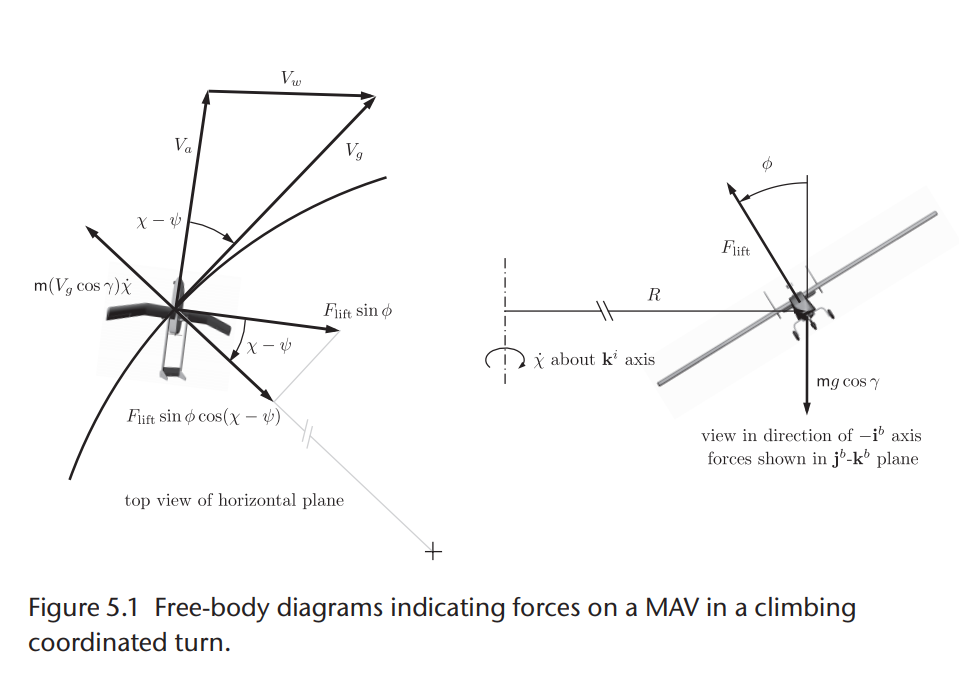
\includegraphics[width=0.8\textwidth]{pictures/5_1.png}
        \caption{爬升协调转弯MAV上的力}
        \label{fig:1}
    \end{figure}
    \par 作用在水平方向力的关系表示如下: 
    \begin{align}
        F_{lift} sin \phi cos (\chi - \psi) &= m \frac{v^{2}}{R} \nonumber \\
        &= m v \omega \nonumber \\
        &= m (V_{g} cos \gamma) \dot{\chi} 
        \label{equ:1}
    \end{align}
    其中, $F_{lift}$代表的是升力, $\gamma$ 代表的是飞行轨迹的角度, $V_{g}, \chi$ 分别表示的是地速度以及方向角. \textcolor{red}{向心加速度的表达式: $a_{n} = \frac{v^{2}}{R} = v \omega$}
    \par 离心力(The centrifugal force)(\textcolor{red}{$m (V_{g} cos \gamma) \dot{\chi} $})计算的时候, 用到了在惯性坐标系$k^{i}$上的方向角变化率$\dot{\chi}$ 和 速度的水平分量 $V_{a}cos \gamma$
    \par 同样, 升力的垂直分量与重力在 $j^{b} - k^{b}$平面上的投影是等大反向的. 
    垂直方向上的合力为:
    \begin{equation}
        F_{lift} cos \phi = mg cos\gamma
        \label{equ:2}
    \end{equation}
    将等式\ref{equ:1}除以\ref{equ:2}得的 $\dot{\chi}$
    \begin{equation}
        \dot{\chi} = \frac{g}{V_{g}} tan \phi cos(\chi - \psi)
        \label{equ:3}
    \end{equation}
    等式\ref{equ:3}就是协调转弯的表达式. 
    \par 考虑到转弯半径等于 \textcolor{blue}{ $R = V_{g} \frac{cos \gamma}{\dot{\chi}}$}, 将上式代入半径中, 得到式子\ref{equ:4}. 在没有风或侧滑的情况下, 有\textcolor{red}{$V_{a} = V_{g}$和$\psi = \chi$}, 从而得到了式子\ref{equ:5}. 
    \begin{equation}
        R = \frac{V_{g}^{2} cos \gamma}{g tan \phi cos(\chi - \psi)} 
        \label{equ:4}
    \end{equation}
    \begin{equation}
        \dot{\chi} = \frac{g}{V_{g}} tan \phi = \dot{\psi} = \frac{g}{V_{a}} tan \phi
        \label{equ:5}
    \end{equation}
    \par 在 9.2 节中, 我们将要介绍 在有风的情况下 \textcolor{blue}{$ \dot{\psi} = \frac{g}{V_{a}} tan \phi$} 该式子也成立
    
    \section{Kinematic Model of Controlled Flight}
    % 控制飞行动力学模型\par
    % 在推导降阶表达式中, 简化的目的是估计运动中力平衡以及动量平衡的关系式(这些包含了 $\dot{u}, \dot{v}, \dot{\omega}, \dot{p}, , \dot{q}, \dot{r}$), 预估这些变量需要计算复杂的空气动力. 这些变量表达式可以被更简单的动力学表达式替代. 
    % 这个更简单的动力学表达式是\textcolor{blue}{针对协调转弯和加速爬升的特定飞行条件而导出}.
    \begin{figure}[htpb]
        \centering
        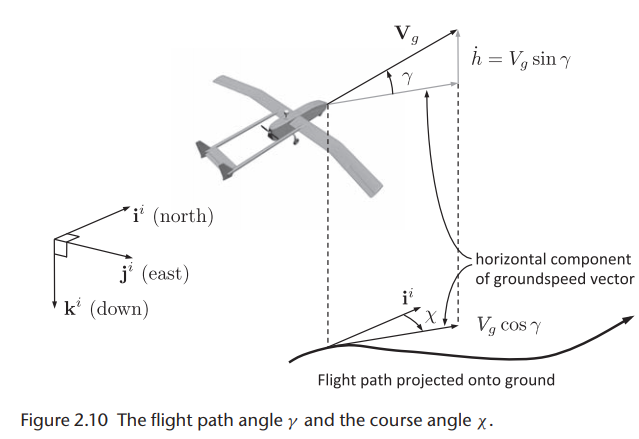
\includegraphics[width=0.8\textwidth]{pictures/2_10.png}
        \caption{航线轨迹角度$\gamma$和航向角$\chi$}
        \label{fig:2_10}
    \end{figure}
    针对图\ref{fig:2_10}, 飞机相对于惯性系的速度矢量可以用航向角和(惯性参考)飞行路径角表示为 
    \begin{gather} % 输入多行公式
        V_{g}^{i} = V_{g} \begin{pmatrix}
            cos \chi cos \gamma \\
            sin \chi cos \gamma \\
            -sin \gamma \\
          \end{pmatrix}
          = \begin{pmatrix}
            \dot{p_{n}} \\
            \dot{p_{e}} \\
            \dot{h} \\
          \end{pmatrix}
          \label{equ:6}
      \end{gather}
    \par 由于控制飞机的航向和空速是很常见的,因此用$\psi$和$V_{a}$表示等式\ref{equ:6}很有用. 
    \begin{gather} % 输入多行公式
        V_{g} \begin{pmatrix}
            cos \chi cos \gamma \\
            sin \chi cos \gamma \\
            -sin \gamma \\
          \end{pmatrix} - \begin{pmatrix}
            w_{n} \\
            w_{e} \\
            w_{d} \\
          \end{pmatrix} =  V_{a} \begin{pmatrix}
            cos \psi cos \gamma_{a} \\
            sin \psi cos \gamma_{a} \\
            -sin \gamma_{a} \\
          \end{pmatrix}
          \label{equ:wind}
      \end{gather}
      结合风的表达式\ref{equ:wind}(地速等于空速加风速, 
        其中的 $\gamma_{a}$ 代表的是 空速的方向和水平方向的夹角), 我们可以得到
      \begin{gather} % 输入多行公式
        \begin{pmatrix}
            \dot{p_{n}} \\
            \dot{p_{e}} \\
            \dot{h} \\
          \end{pmatrix} = V_{a} \begin{pmatrix}
            cos \psi cos \gamma_{a} \\
            sin \psi cos \gamma_{a} \\
            sin \gamma_{a} \\
          \end{pmatrix} +  \begin{pmatrix}
            w_{n} \\
            w_{e} \\
            -w_{d} \\
          \end{pmatrix}
          \label{equ:7}
      \end{gather}
      如果我们假设飞机保持在一个恒定的高度,并且没有向下的风分量,那么运动学表达式简化为\ref{equ:8}, 同样该模型也是无人机领域中比较常用的模型. 
      \begin{gather} % 输入多行公式
        \begin{pmatrix}
            \dot{p_{n}} \\
            \dot{p_{e}} \\
            \dot{h} \\
          \end{pmatrix} = V_{a} \begin{pmatrix}
            cos \psi \\
            sin \psi \\
            0 \\
          \end{pmatrix} +  \begin{pmatrix}
            w_{n} \\
            w_{e} \\
            0 \\
          \end{pmatrix}
          \label{equ:8}
      \end{gather}
      \subsection{Coordinated Turn}
      之前的协调转弯的表达式为 $\dot{\chi} = \frac{g}{V_{g}} tan \phi cos(\chi - \psi)$. 
      即使在第6章中描述的自动驾驶回路并没有强制执行协调转弯条件,
      飞机必须倾斜才能转弯(而不是打滑才能转弯)这个基本条件已经被这个模型捕捉到了。\par
      协调转弯可以被 heading 和 空速进行表示. 我们先对\ref{equ:wind}两边进行求导, 得到下面的式子\ref{equ:9}
      \begin{gather} % 输入多行公式
        \begin{pmatrix}
            cos \chi cos \gamma & - V_{g} sin \chi cos \gamma & - V_{g} cos \chi sin \gamma \\
            sin \chi cos \gamma & V_{g} cos \chi cos \gamma & - V_{g} sin \chi sin \gamma \\
            -sin \gamma & 0 & -cos \gamma \\
          \end{pmatrix} \begin{pmatrix}
            \dot{V_{g}} \\
            \dot{\chi} \\
            \dot{\gamma} \\
        \end{pmatrix}
          = \begin{pmatrix}
            cos \psi cos \gamma_{a} & - V_{a} sin \psi cos \gamma_{a} & - V_{a} cos \psi sin \gamma_{a} \\
            sin \psi cos \gamma_{a} & V_{a} cos \psi cos \gamma_{a} & - V_{a} sin \psi sin \gamma_{a} \\
            -sin \gamma_{a} & 0 & -cos \gamma_{a} \\
          \end{pmatrix} \begin{pmatrix}
            \dot{V_{a}} \\
            \dot{\psi} \\
            \dot{\gamma_{a}} \\
        \end{pmatrix}
          \label{equ:9}
      \end{gather}
      \par 在定高和没有向下风分量的情况下, $\gamma, \gamma_{a}, \dot{\gamma}, \dot{\gamma_a}$ 和 $w_{d}$ 都是0, 根据$\dot{V_{a}}$ 和$\dot{\chi}$求解$\dot{V_{g}}$ 和$\dot{\psi}$
      \begin{equation}
        \begin{split}
          \dot{V_{g}} &= \frac{\dot{V_{a}}}{cos (\chi - \psi)} + V_{g} \dot{\chi} tan(\chi - \psi) \\
          \dot{\psi} &= \frac{\dot{V_{a}}}{V_{a}} tan (\chi - \psi) + \frac{V_{g} \dot{\chi}}{V_{a}cos(\chi - \psi)}
        \end{split}
    \end{equation}
    \par 若假定空速为常数, 那么得\ref{equ:10} 最值得注意的是在有风的情况下,这个等式是成立的。
    \begin{equation}
        \dot{\chi} = \frac{g}{V_{g}} tan \phi 
        \label{equ:10}
    \end{equation}
    \subsection{Accelerating Climb}
\end{document}